
\section{Discussion and Future Work}

While \lib{} makes significant improvements over prior systems, there are some types of workloads that \lib{} (and all current TSO deterministic systems) will struggle to support efficiently. One such class of programs is those that use fine-grained locking with relatively short chunk sizes. In \lib{}, each lock and unlock will be totally ordered and will require a global commit operation. This significantly impacts scalability, as was seen in the {\it water\_nsquared} benchmark program. 

This is one class of programs where relaxed consistency can make an improvement over TSO. In an LRC system, the lock acquisitions and releases must still be totally ordered but the commit operations can be done in parallel for distinct locks. Therefore, even if the total amount of memory that must be propagated between threads for the two consistency models is roughly the same, the LRC system may exhibit better scalability. In our future work, we look to better support these types of workloads while maintaining TSO.

\begin{figure}
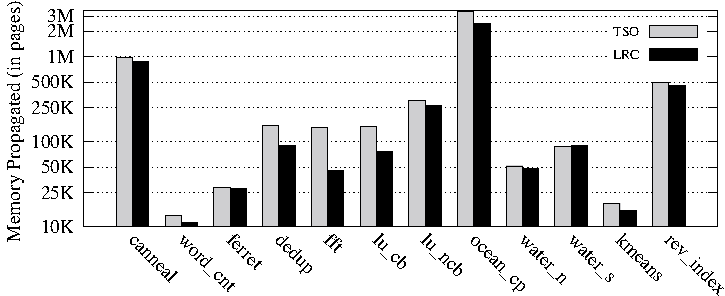
\includegraphics[width=3.3in]{figures/tso_vs_lrc.pdf}
\caption{Total pages propagated under TSO (\lib{}) and the expected number for an LRC-based system. (log scale y)}
\label{f:tsovslrc}
\end{figure}

